\begin{UseCase}{CU1.1.3}{Eliminar productos del carrito} { %Luis 
Resumen:El empleado eliminara los productos que el cliente ya no desee comprar o que no pueda comprar,cabe resaltar que para eliminar los productos no se ocupará ninguna base de datos, los datos solo estarán en el front de la pagina.
}
	
\UCitem{Versión}{1.0}
\UCccsection{Administración}
\UCccitem{Autor}{Vazquez Ortiz Luis Enrique}
\UCccitem{Evaluador}{}
\UCccitem{Operación}{}
\UCccitem{Prioridad}{Alta}
\UCccitem{Complejidad}{Media}
\UCccitem{Volatilidad}{Baja}
\UCccitem{Madurez}{Alta}
\UCccitem{Estatus}{Edición}
\UCccitem{Fecha del último estatus}{17 de Diembre del 2021}

%% Copie y pegue este bloque tantas veces como revisiones tenga el caso de uso.
%% Esta sección la debe llenar solo el Revisor
% %--------------------------------------------------------
	%   % Revisión Versión (Anote la versión que se revisó.)
\UCccsection{Revisión Versión 0.1 }
% 	% FECHA: Anote la fecha en que se terminó la revisión.
\UCccitem{Fecha}{} 
% 	% EVALUADOR: Coloque el nombre completo de quien realizó la revisión.
\UCccitem{Evaluador}{}
% 	% RESULTADO: Coloque la palabra que mas se apegue al tipo de acción que el analista debe realizar.
\UCccitem{Resultado}{}
% 	% OBSERVACIONES: Liste los cambios que debe realizar el Analista.
\UCccitem{Observaciones}{
	\begin{UClist}
		%\RCitem{PC1}{\DONE{En la pantalla falta el botón del ojito}}{18 de Abril del 2018}
	\end{UClist}		
}

% %--------------------------------------------------------
	
\UCsection{Atributos}
	\UCitem{Actor(es)}{
		\cdtRef{Actor:RT}{Empleado} 
	}
	\UCitem{Propósito}{
		Eliminar los procductos que se encuentran en el carrito.
	}
	\UCitem{Entradas}{
		Nombre del medicamento.
	}
	\UCitem{Salidas}{
		
		\begin{UClist}
		Ninguna
							
		\end{UClist}
	}

	\UCitem{Precondiciones}{. 
		\UCli El producto debe estar previamente ingresado en el sistema
	}
	\UCitem{Postcondiciones}{
		Ninguna
	}
	\UCitem{Reglas de negocio}{
		Ninguna
	}
	\UCitem{Errores}{
		Ninguna
	}
	\UCitem{Tipo}{}
\end{UseCase}

\begin{UCtrayectoria}
	
	\UCpaso[\UCactor] Selecciona icono de basura para eliminar algún prodcuto del carrito.
	
	\UCpaso[\UCsist]Muestra una pantalla emergente- "Cuidado! ¿Seguro que desea eliminar los productos?"

	\UCpaso[\UCactor] Selecciona la opción \cdtButton{SI}\refTray{A} 

	\UCpaso[\UCsist]Elimina el o los productos del carrito.

	\UCpaso[\UCsist] Muestra " Producto(s) eliminado(s) con éxito!"

	\UCpaso[\UCsist]Muestra la página de |Ventas|


	
\end{UCtrayectoria}


%...........::::::::::::TRAYECTORIAS ALTERNATIVAS::::::::::::::........
%-------------------------Trayectoria A------------------------------
\begin{UCtrayectoriaA}{A}{No se elima el prodcuto del carrito}

	\UCpaso[\UCactor] Presiona el botón \cdtButton{No}.
	
	\UCpaso[\UCsist]Cierra la ventana emergente.

	\UCpaso[\UCsist]Muestra la página de |Ventas|.
	
\end{UCtrayectoriaA}

{
\begin{flushleft}
	\break


	% Secuencia
	\Large{Secuencia}\\
	\rule{14cm}{0.5pt}

	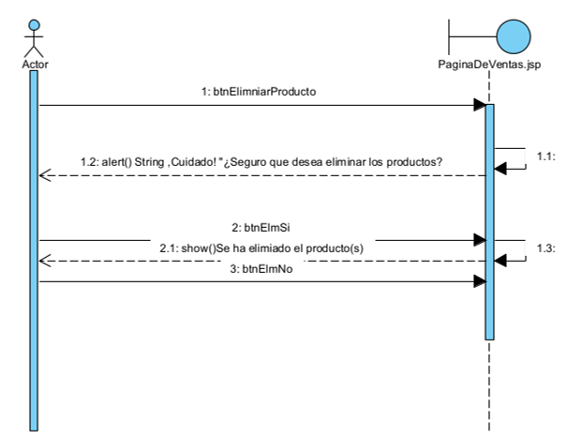
\includegraphics[height=8cm]{casouso/cu10/images/Diagram_Sequence.png}\\	
	
	
\end{flushleft}
}
